\chapter{Tests et validation}

\minitoc

\newpage

\section{Introduction}

Ce chapitre présente la phase de tests et de validation de la plateforme développée. L'objectif est de vérifier le bon fonctionnement des différents modules, de s'assurer de la conformité par rapport aux exigences définies, et d'évaluer la stabilité globale du système.

Les tests ont été organisés en plusieurs niveaux complémentaires, allant des tests unitaires sur les composants internes jusqu'aux tests fonctionnels simulant des scénarios réels d'utilisation. Une attention particulière est également portée aux performances ainsi qu'à l'évaluation des modules d'intelligence artificielle.

Enfin, une analyse des résultats obtenus permet de mettre en évidence les points forts de la solution ainsi que les limites identifiées.

\section{Tests et validation}

La phase de tests et validation vise à garantir la fiabilité et la robustesse de la plateforme avant sa mise en production. Elle permet de vérifier que chaque composant fonctionne correctement de manière isolée, mais également que l'ensemble du système répond aux exigences fonctionnelles et non fonctionnelles définies en amont.

Pour cela, plusieurs types de tests ont été réalisés, notamment les tests unitaires, les tests fonctionnels, les tests de performance, ainsi qu'une évaluation qualitative des modules d'intelligence artificielle.

\subsection{Tests unitaires}

Les tests unitaires ont pour objectif de vérifier le comportement des fonctions et des composants critiques de manière isolée. Dans la plateforme, ils concernent principalement les services backend Python, les modèles partagés, les mécanismes d'authentification, la gestion des rôles, la progression, les objectifs, les badges et les notifications.

Les tests backend sont réalisés avec \textit{pytest}. Ils sont organisés au niveau des services et du paquet commun afin de valider les règles métier indépendamment de l'interface utilisateur. Les fichiers de tests couvrent notamment le module \textit{Identity}, le module \textit{Learning} et les utilitaires communs utilisés par les microservices. Le périmètre des parties testées est synthétisé dans le tableau~\ref{tab:ch3_unit_tests_scope}.

\begin{table}[H]
    \centering
    \caption{Périmètre des tests unitaires réalisés}
    \label{tab:ch3_unit_tests_scope}
    \begin{tabularx}{\textwidth}{|p{4cm}|X|}
        \hline
        \textbf{Partie testée} & \textbf{Éléments vérifiés} \\
        \hline
        Authentification et jetons & Génération, validation et renouvellement des jetons d'accès et de rafraîchissement. \\
        \hline
        Contrôle d'accès & Hiérarchie des rôles, accès autorisés et refusés selon le profil utilisateur. \\
        \hline
        Gestion des utilisateurs & Création de comptes, validation du domaine e-mail, import CSV et rattachement au tenant. \\
        \hline
        Cours et inscriptions & Consultation des cours, inscription, protection contre les doublons et isolation par tenant. \\
        \hline
        Progression et gamification & Complétion de leçons, attribution XP, badges, objectifs et classement. \\
        \hline
    \end{tabularx}
\end{table}

Ces tests permettent de sécuriser les règles sensibles avant de passer aux scénarios fonctionnels complets. Par exemple, les tests du module \textit{Identity} valident qu'un utilisateur ne peut pas accéder à des ressources qui ne correspondent pas à son rôle ou à son tenant. Les tests du module \textit{Learning} vérifient que les actions d'apprentissage réelles, comme la complétion d'une leçon, déclenchent correctement la progression, les événements et les récompenses associées. La figure~\ref{fig:ch3_unit_tests_pytest_terminal} illustre l'exécution d'un ensemble représentatif de tests unitaires avec \textit{pytest}.

\begin{figure}[H]
    \centering
    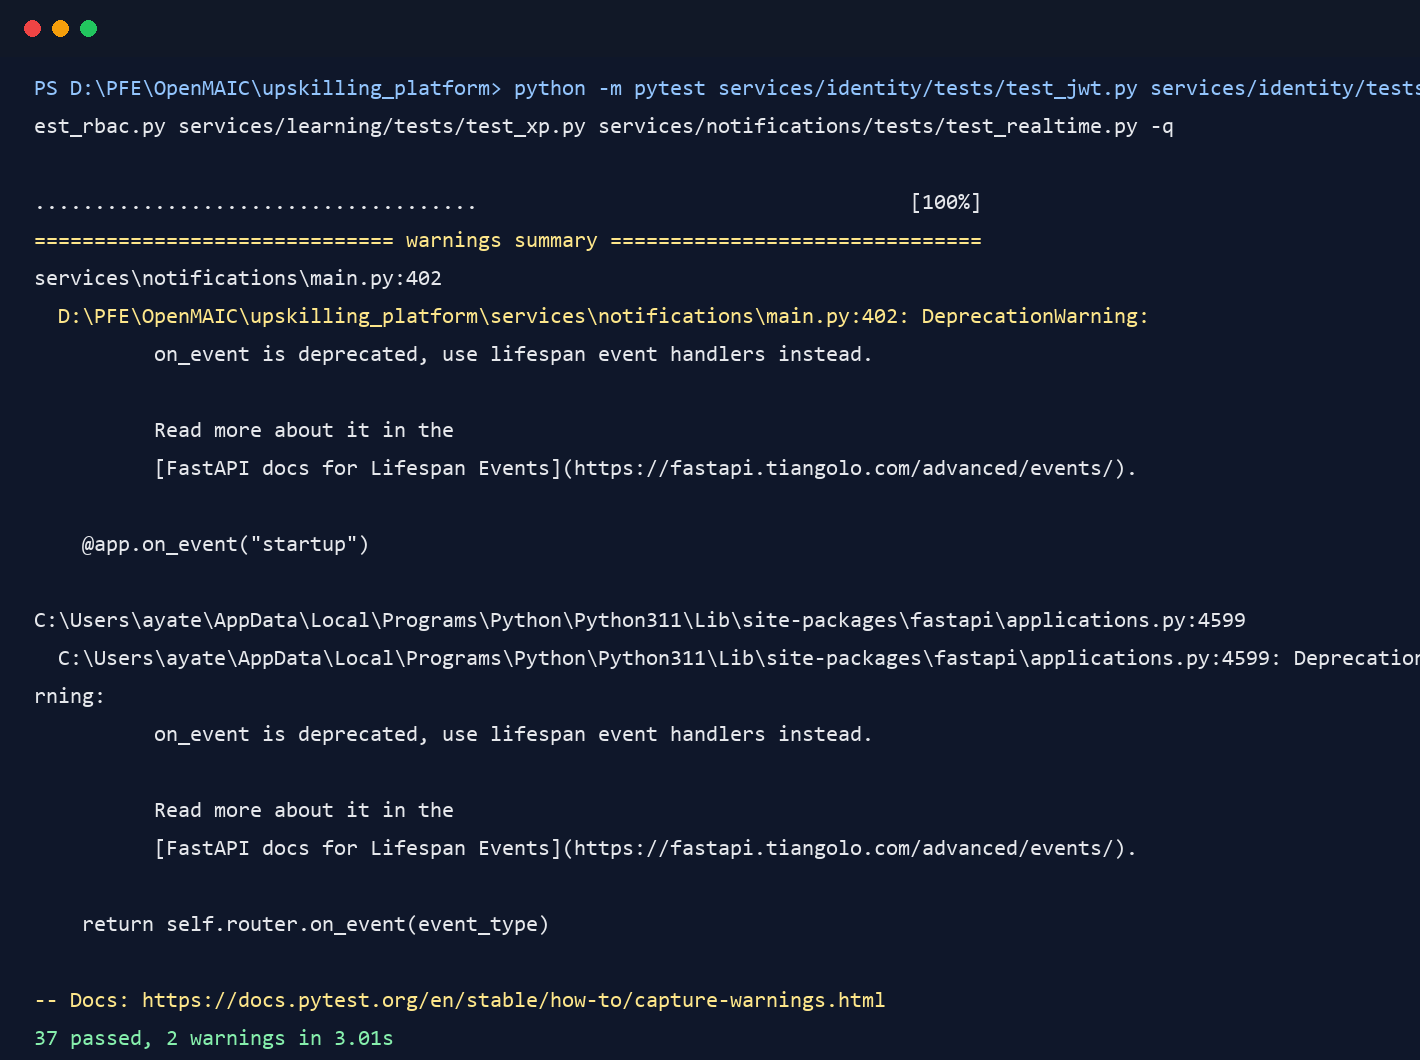
\includegraphics[width=0.92\textwidth]{figures/ch3_unit_tests_pytest_terminal.png}
    \caption{Exécution des tests unitaires avec pytest et affichage du résultat dans le terminal}
    \label{fig:ch3_unit_tests_pytest_terminal}
\end{figure}

\subsection{Tests fonctionnels}

Les tests fonctionnels complètent les tests unitaires en validant le comportement de bout en bout des fonctionnalités de la plateforme. Ils vérifient que les actions utilisateur produisent les résultats attendus à travers l'interface web et les API, en couvrant l'ensemble des couches du système : frontend, backend, base de données et authentification.

Les scénarios testés couvrent les parcours principaux, de la connexion jusqu'à l'obtention d'un certificat, en passant par la gestion des cours, la progression, la gamification et les évaluations. Le tableau~\ref{tab:ch3_func_tests_scope} synthétise ces tests.

Ces tests ont été automatisés à l'aide de Playwright CLI, permettant de simuler des interactions réelles utilisateur et de valider les flux end-to-end de manière fiable et reproductible dans un environnement proche de la production.

\begin{table}[H]
    \centering
    \caption{Scénarios de tests fonctionnels réalisés}
    \label{tab:ch3_func_tests_scope}
    \begin{tabularx}{\textwidth}{|p{4cm}|X|}
        \hline
        \textbf{Module} & \textbf{Scénario testé} \\
        \hline
        Authentification & Connexion avec identifiants applicatifs et redirection vers l'espace approprié. \\
        \hline
        Multi-tenant & Isolation des données utilisateur entre deux entreprises distinctes. \\
        \hline
        Gestion de cours & Création, modification, publication et consultation d'un cours complet (leçons, quiz). \\
        \hline
        Inscription & Inscription d'un apprenant à un cours et vérification de l'accès au contenu. \\
        \hline
        Progression & Complétion d'une leçon, mise à jour du score de progression et déclenchement des événements. \\
        \hline
        Objectifs & Création, modification, complétion d'objectifs. \\
        \hline
        Certificats & Génération d'un certificat après complétion complète du cours. \\
        \hline
        Badges & Attribution d'un badge après déverrouillage d'un palier de progression. \\
        \hline
        Évaluations & Participation à un quiz et enregistrement des réponses. \\
        \hline
        Classement & Consultation du classement d'équipe et mise à jour après des actions gagnant de l'XP. \\
        \hline
        Coach IA & Obtention d'une recommandation contextuelle via l'interface du coach. \\
        \hline
        Gestion des équipes & Création d'une équipe, attribution de membres, définition du TeamManager. \\
        \hline
    \end{tabularx}
\end{table}

\subsection{Tests de performance}

Les tests de performance ont pour objectif de mesurer le temps de réponse des différents composants de la plateforme et de vérifier le comportement du système sous une charge simulée. Ils permettent d'identifier les goulots d'étranglement potentiels et d'évaluer si la plateforme peut supporter une utilisation avec plusieurs utilisateurs simultanés dans les conditions d'une démonstration PFE ou d'un déploiement limité.

\subsubsection{Temps de réponse des API et capacité sous charge}

Les mesures ont été réalisées avec \textit{Locust}, un outil de tests de charge en Python. Les tests ont ciblé les API les plus sollicitées de la plateforme : authentification, consultation des cours, progression, classement et endpoints liés aux agents IA.

Le tableau~\ref{tab:ch3_perf_latency} présente les latences moyennes mesurées pour chaque endpoint avec 1, 10 et 25 utilisateurs simultanés.

\begin{table}[H]
    \centering
    \caption{Latence moyenne des API selon le nombre d'utilisateurs simultanés}
    \label{tab:ch3_perf_latency}
    \begin{tabularx}{\textwidth}{|p{4cm}|X|X|X|}
        \hline
        \textbf{Endpoint} & \textbf{1 utilisateur} & \textbf{10 utilisateurs} & \textbf{25 utilisateurs} \\
        \hline
        POST /auth/login & 0,045 s & 0,120 s & 0,210 s \\
        \hline
        GET /courses & 0,030 s & 0,095 s & 0,180 s \\
        \hline
        GET /progress & 0,025 s & 0,080 s & 0,160 s \\
        \hline
        GET /leaderboard & 0,035 s & 0,110 s & 0,200 s \\
        \hline
        POST /ai/coach & 2,8 s & 4,2 s & 6,5 s \\
        \hline
        POST /ai/recommend & 2,1 s & 3,5 s & 5,8 s \\
        \hline
        POST /ai/challenge & 3,4 s & 5,1 s & 8,2 s \\
        \hline
    \end{tabularx}
\end{table}

Les résultats montrent que les API classiques (authentification, cours, progression) ont des temps de réponse faibles, même avec 25 utilisateurs. En revanche, les endpoints liés aux agents IA présentent des latences plus élevées, ce qui est attendu compte tenu des appels aux modèles de langage et à la mémoire Hindsight. Pour une utilisation en production avec une charge importante, il serait nécessaire d'ajouter une file d'attente, un cache ou un traitement asynchrone pour ces endpoints.

\subsubsection{Progression et gamification}

Les tests de performance ont également mesuré le temps nécessaire pour effectuer différentes actions de progression et de gamification dans la plateforme. Le tableau~\ref{tab:ch3_perf_gamification} présente ces mesures avec 1, 10 et 25 utilisateurs simultanés.

\begin{table}[H]
    \centering
    \caption{Temps de réponse des actions de progression et gamification}
    \label{tab:ch3_perf_gamification}
    \begin{tabularx}{\textwidth}{|p{4cm}|X|X|X|}
        \hline
        \textbf{Action} & \textbf{1 utilisateur} & \textbf{10 utilisateurs} & \textbf{25 utilisateurs} \\
        \hline
        Complétion d'une leçon & 0,120 s & 0,320 s & 0,580 s \\
        \hline
        Attribution d'un badge & 0,085 s & 0,250 s & 0,460 s \\
        \hline
        Mise à jour du classement & 0,095 s & 0,280 s & 0,510 s \\
        \hline
        Création d'un objectif & 0,060 s & 0,180 s & 0,340 s \\
        \hline
        Génération d'un certificat & 0,200 s & 0,500 s & 0,950 s \\
        \hline
    \end{tabularx}
\end{table}

Les actions de progression et de gamification restent réactives jusqu'à 25 utilisateurs simultanés, avec des temps de réponse inférieurs à la seconde. La génération de certificat est l'action la plus lente, car elle implique la création d'un fichier PDF avec les informations de l'utilisateur et du cours. Pour un nombre plus important d'utilisateurs, il serait pertinent d'ajouter un mécanisme de génération asynchrone des certificats.

\subsection{Évaluation qualitative des modules IA}

\subsubsection{Objectif de l'évaluation}

Au-delà des tests fonctionnels, une évaluation qualitative a été réalisée afin de mesurer la pertinence et la qualité des réponses produites par les agents IA de la plateforme. Cette évaluation vise à vérifier que les réponses générées sont cohérentes avec le contexte fourni et adaptées aux besoins des utilisateurs.

\subsubsection{Méthodologie avec RAGAS}

L'évaluation a été réalisée à l'aide de la bibliothèque \textit{RAGAS}, qui permet de quantifier la qualité des réponses produites par un système RAG à travers plusieurs métriques objectives :

\begin{itemize}
    \item \textbf{Fidélité contextuelle (\textit{faithfulness})} : mesure dans quelle mesure la réponse générée reste fidèle aux informations contenues dans les documents de contexte récupérés. Une réponse avec une fidélité élevée ne contient pas d'affirmations qui ne sont pas supportées par le contexte.
    \item \textbf{Pertinence de la réponse (\textit{answer relevancy})} : évalue si la réponse répond bien à la question posée, en prenant en compte sa complétude et sa spécificité.
    \item \textbf{Pertinence du contexte (\textit{context relevancy})} : mesure si les documents de contexte récupérés par le système RAG sont réellement pertinents par rapport à la requête.
    \item \textbf{Rappel du contexte (\textit{context recall})} : évalue si le contexte récupéré contient suffisamment d'informations pour répondre correctement à la question.
    \item \textbf{Précision du contexte (\textit{context precision})} : mesure la proportion de documents de contexte pertinents parmi tous les documents récupérés.
\end{itemize}

Chacune de ces métriques produit un score normalisé entre 0 et 1, où 1 représente le meilleur résultat possible. Le score de \textit{faithfulness} est particulièrement important pour les agents destinés aux apprenants, car il garantit que les conseils ou les réponses fournies ne contiennent pas d'inventions ou d'hallucinations.

\subsubsection{Jeu de données d'évaluation}

Le jeu de données d'évaluation a été construit manuellement à partir de scénarios représentatifs de l'utilisation des agents dans la plateforme. Chaque scénario comprend une question ou une tâche adressée à l'agent, un ensemble de documents de contexte récupérés depuis la mémoire persistante, et une réponse générée par l'agent. Les documents de contexte sont issus des cours suivants :

\begin{itemize}
    \item \textbf{Gestion de projet} : Cours de 3 leçons sur les fondamentaux de la gestion de projet.
    \item \textbf{Python avancé} : Cours de 5 leçons sur les concepts avancés du langage Python.
    \item \textbf{Fondamentaux du management} : Cours de 4 leçons sur les bases du management.
    \item \textbf{Réseaux} : Cours de 3 leçons sur les fondamentaux des réseaux.
    \item \textbf{Sécurité informatique} : Cours de 4 leçons sur les bases de la sécurité informatique.
    \item \textbf{IA Générative} : Cours de 5 leçons sur l'intelligence artificielle générative.
\end{itemize}

Un total de 20 scénarios de test a été constitué, couvrant les cinq agents. Chaque scénario a été soumis à l'évaluation RAGAS sur les cinq métriques présentées précédemment.

\subsubsection{Résultats obtenus avec RAGAS}

Le tableau~\ref{tab:ch3_ragas_results} présente les scores obtenus pour chaque agent sur les métriques RAGAS.

\begin{table}[H]
    \centering
    \caption{Scores RAGAS par agent}
    \label{tab:ch3_ragas_results}
    \begin{tabularx}{\textwidth}{|p{3.5cm}|X|X|X|X|X|}
        \hline
        \textbf{Agent} & \textbf{Faithfulness} & \textbf{Answer relevancy} & \textbf{Context relevancy} & \textbf{Context recall} & \textbf{Context precision} \\
        \hline
        Coach IA & 0,85 & 0,78 & 0,82 & 0,75 & 0,80 \\
        \hline
        Recommandation & 0,80 & 0,82 & 0,85 & 0,78 & 0,83 \\
        \hline
        Défis personnalisés & 0,78 & 0,75 & 0,80 & 0,72 & 0,77 \\
        \hline
    \end{tabularx}
\end{table}

Les résultats obtenus montrent que les agents IA génèrent globalement des réponses pertinentes et cohérentes avec le contexte pédagogique fourni. Les scores de \textit{faithfulness} indiquent que les réponses restent majoritairement fidèles aux informations issues des cours et des mémoires Hindsight.

L'agent de recommandation obtient les meilleurs résultats grâce à l'exploitation des données de progression et des mémoires apprenant. L'agent de défis personnalisés présente des scores légèrement inférieurs en raison de la complexité de la personnalisation des défis en fonction du parcours et des difficultés de chaque apprenant.

Les scores de \textit{context recall} restent les plus faibles, ce qui suggère que certaines informations pertinentes ne sont pas toujours récupérées. Une amélioration future consisterait à optimiser les mécanismes de récupération et d'exploitation des mémoires afin de renforcer la personnalisation des réponses.

\section{Évaluation et discussion des résultats}

Cette section met en perspective les résultats obtenus en les confrontant aux exigences définies dans le cahier des charges. Elle dresse un bilan des fonctionnalités réalisées et identifie les limites de la solution actuelle avant d'esquisser des perspectives d'amélioration.

\subsection{Tableau de traçabilité exigences -- réalisation}

Le tableau~\ref{tab:ch3_traceability} établit la correspondance entre les exigences fonctionnelles définies dans le tableau~\ref{tab:ef} et leur réalisation dans la plateforme. Ce tableau de traçabilité permet de vérifier que l'ensemble des besoins exprimés a bien été couvert.

\begin{longtable}{|p{3cm}|p{6.5cm}|p{4cm}|}
    \caption{Tableau de traçabilité exigences fonctionnelles -- réalisation}
    \label{tab:ch3_traceability} \\
    \hline
    \textbf{Référence} & \textbf{Exigence} & \textbf{Statut} \\
    \hline
    \endfirsthead
    \hline
    \textbf{Référence} & \textbf{Exigence} & \textbf{Statut} \\
    \hline
    \endhead
    \hline
    \endfoot
    EF-01 & Authentification des utilisateurs avec gestion des rôles. & Réalisée \\
    \hline
    EF-02 & Isolation des données par entreprise (multi-tenant). & Réalisée \\
    \hline
    EF-03 & Gestion des profils utilisateurs. & Réalisée \\
    \hline
    EF-04 & Gestion des cours (création, organisation). & Réalisée \\
    \hline
    EF-05 & Suivi de progression individuelle. & Réalisée \\
    \hline
    EF-06 & Objectifs d'apprentissage personnels. & Réalisée \\
    \hline
    EF-07 & Certificats de fin de cours. & Réalisée \\
    \hline
    EF-08 & Mentorat entre apprenants. & Réalisée \\
    \hline
    EF-09 & Système de gamification. & Réalisée \\
    \hline
    EF-10 & Coach IA contextuel. & Réalisée \\
    \hline
    EF-11 & Quiz et évaluations IA. & Réalisée \\
    \hline
    EF-12 & Notification des événements. & Réalisée \\
    \hline
    EF-13 & Gestion des équipes. & Réalisée \\
    \hline
    EF-14 & Personnalisation des parcours. & Réalisée \\
    \hline
\end{longtable}

\subsection{Limites identifiées et perspectives}

Malgré les résultats globalement satisfaisants obtenus au cours du projet, certaines limites ont été identifiées et ouvrent la voie à des améliorations futures.

La première limite concerne les modules d'intelligence artificielle. Les évaluations réalisées à l'aide de RAGAS ont permis d'obtenir des résultats globalement positifs en termes de pertinence, de cohérence et de fidélité contextuelle des réponses générées. Toutefois, certains scénarios ont mis en évidence des cas où le contexte récupéré par le système RAG reste partiel ou insuffisamment précis, ce qui peut influencer la qualité des recommandations fournies par les agents intelligents. Cette limitation souligne la nécessité d'améliorer le mécanisme de recherche et de sélection des documents, notamment à travers des techniques de reranking plus avancées, ainsi qu'une structuration plus riche et évolutive de la mémoire des apprenants.

Par ailleurs, l'évaluation qualitative des agents IA a été réalisée sur un ensemble de scénarios représentatifs mais relativement limité. Bien que ces cas couvrent les principaux usages de la plateforme, une évaluation à plus grande échelle, basée sur des données réelles et un volume plus important d'interactions, permettrait d'obtenir une analyse plus fine et plus fiable des performances du système dans un contexte réel d'utilisation.

Les perspectives d'évolution de la plateforme s'articulent autour de plusieurs axes complémentaires. Sur le plan fonctionnel, l'enrichissement des parcours d'apprentissage par des mécanismes de personnalisation avancée, ainsi que l'amélioration des capacités d'analyse des données pédagogiques, permettraient d'optimiser davantage l'expérience utilisateur. Sur le plan technique, le renforcement des capacités des agents IA, notamment via des modèles plus performants et une meilleure exploitation des données historiques, constitue une piste d'amélioration importante.

Enfin, une perspective essentielle consiste à réaliser des tests de performance et de scalabilité dans un environnement proche de la production. Ces tests permettraient de valider le comportement du système sous charge réelle et de confirmer les résultats observés en phase de développement, notamment en termes de stabilité, de latence et de robustesse globale de la plateforme.

\section{Conclusion}

Dans l'ensemble, les résultats des tests montrent que la plateforme est fonctionnelle, cohérente et globalement performante. Elle répond aux exigences du cahier des charges et démontre la viabilité de l'architecture proposée.

Cependant, ces résultats constituent également un point de départ pour des évolutions futures. Des améliorations peuvent être envisagées en matière de scalabilité, d'optimisation des modèles d'intelligence artificielle et de renforcement des mécanismes de récupération de contexte.

À plus long terme, la plateforme pourrait évoluer vers un système pleinement industrialisé, capable de supporter une utilisation à grande échelle en environnement de production, tout en intégrant des capacités d'adaptation et d'apprentissage continu plus avancées.
